\section{Описание проекта}
\subsection{Структура проекта}
Проект состоит из пяти страниц:
\begin{enumerate}
  \item Первый экран
  \item Наши преимущества
  \item Услуги
  \item Портфолио
  \item Тест. Узнайте какой тип сайта больше всего подходит вам
\end{enumerate}
\subsection{Структура и описание страниц проекта}

\subsubsection{Первый экран}
\begin{enumerate}
  \item Навигация: Услуги, Портфолио, Контакты;
  \item progress bar ( интерактивная шкала прогресса )
  \item Ссылки на соц. сети: facebook, instagram, vk, github, what's app, telegram;
  \item Логотип: app-jedi;
  \item Уникальное торговое предложение: Разработка эффективных веб-приложений для вашего бизнеса Дополнительно: "Пройдите тест, узнайте какой тип сайта большего всего подходит вам и получите наше уникальное предложение" ;
  \item Кнопка "Пройти тест";
\end{enumerate}

\subsubsection{Наши преимущества}
\begin{enumerate}
  \item Заголовок
  \item Текст
  \item Преимущества в виде инфографики (желательно интерактивной):
  \begin{enumerate}
    \item Эргономичный дизайн
    \item Высокая скорость работы
    \item Автоматизация рутинных процессов
    \item Дружелюбный и отзывчивый дизайн
    \item Масштабируемая архитектура
    \item Адаптивность под любые типы устройств
  \end{enumerate}
\end{enumerate}

\subsubsection{Услуги}
\begin{enumerate}
  \item Основные услуги
  \begin{enumerate}
    \item Разработка лендингов и промо-сайтов
      \paragraph{Описание}: Простота, информативность и невысокая стоимость сделали посадочные страницы самым востребованным форматом веб-приложений для малого и среднего бизнеса. Данное решение отлично подходит для тех, кто продаёт единственный товар, или предоставляется единственную услугу!

    \item Разработка сайтов-визиток
      \paragraph{Описание}: Сайт-визитка отлично тем, кто хочет ограничиться предоставлением информации о себе или своей компании и увеличить лояльность своей аудитории;

    \item Разработка сайтов-резюме
      \paragraph{Описание}: Хотите выделиться из толпы и устроиться на желанную вакансию? Резюме в формате веб-приложения подчеркнёт ваши достоинства, выделит профессиональные компетенции и сделает более привлекательным соискателем для работодателя;

    \item Разработка интернет-магазинов:
      \begin{enumerate}
        \item Интернет-магазины на премиум-шаблоне
        \item Уникальные интернет-магазины
      \end{enumerate}
      \paragraph{Описание}: Хотите начать зарабатывать на электронной коммерции? Воспользуйтесь нашим решением на базе премиум-шаблона, или закажите веб-приложение с уникальными дизайном и модулями.

    \item Разработка онлайн-сервисов \paragraph{Описание}: У вас есть идея веб-приложения? Мы проведём анализ вашей идеи, разработаем приложение и составим план дальнейшего развития.
  \end{enumerate}

  \item Дополнительные услуги
  \begin{enumerate}
    \item Разработка технического задания
      \paragraph{Описание}: Грамотное составление технического задания напрямую влияет на время разработки проекта и его качество. Перенесите все свои мысли и идеи в четкий формализованный документ, содержащий все необходимые условия и требования к разработке, доверив решение данной задачи нашим профессионалам.
    \item Адаптивная верстка вашего проекта
      \paragraph{Описание}: У вас уже есть готовый дизайн сайта? Воспользуйтесь нашей услугой верстки и получИте на выходе шаблон, который будет отлично смотреться на любых устройствах
    \item Интеграция сторонних сервисов
      \paragraph{Описание}: Вам нужно привязать к сайту систему аналитики, интегрировать CRM-систему или настроить сторонний модуль? Мы качественно выполним данную задачу по весьма демократичной цене!
    \item Комплексная поддержка сайта
      \paragraph{Описание}: Не работает форма отправки? Нужно добавить материалы на сайт, почистить код, сделать бэкап, восстановить систему или написать руководство по работе в панели управления? Мы решим вашу проблему в кратчайшие сроки!
  \end{enumerate}

\end{enumerate}

\subsubsection{Портфолио}
\begin{enumerate}
  \item Лендинги и промо-сайты
  \item Резюме
  \item Сайты-визитки
  \item Интернет-магазины
  \item Онлайн-сервисы
\end{enumerate}

\subsubsection{Тест. Узнайте какой тип сайта больше всего подходит вам}
\begin{enumerate}
  \item Кнопка «Начать тест»
  \item Последовательное переключение вопросов с выбором одного, или нескольких вариантов ответа
  \item Граф (дерево) прогресса (при ответе на вопрос подсвечивается одна или другая ветка)
  \begin{enumerate}
    \item Дерево находится сбоку от теста и не включает заголовки (только ветки и точки)
    \item Картинка с примером прилагается
    \item Дерево должно быть аккуратное и красивое
  \end{enumerate}
  \item После прохождения теста появление формы с ответом в формате:
  \begin{enumerate}
    \item Заголовок
    \item Текст ответа
    \item Подзаголовок для предоставления уникального торгового предложения (Оставьте заявку прямо сейчас и получите скидку на разработку Вашего уникального сайта-визитки)
    \item Форма обратной связи: Имя, Номер телефона,
    \item Кнопка «Отправить заявку»
  \end{enumerate}
  Схема теста:
  \begin{figure}[H]
    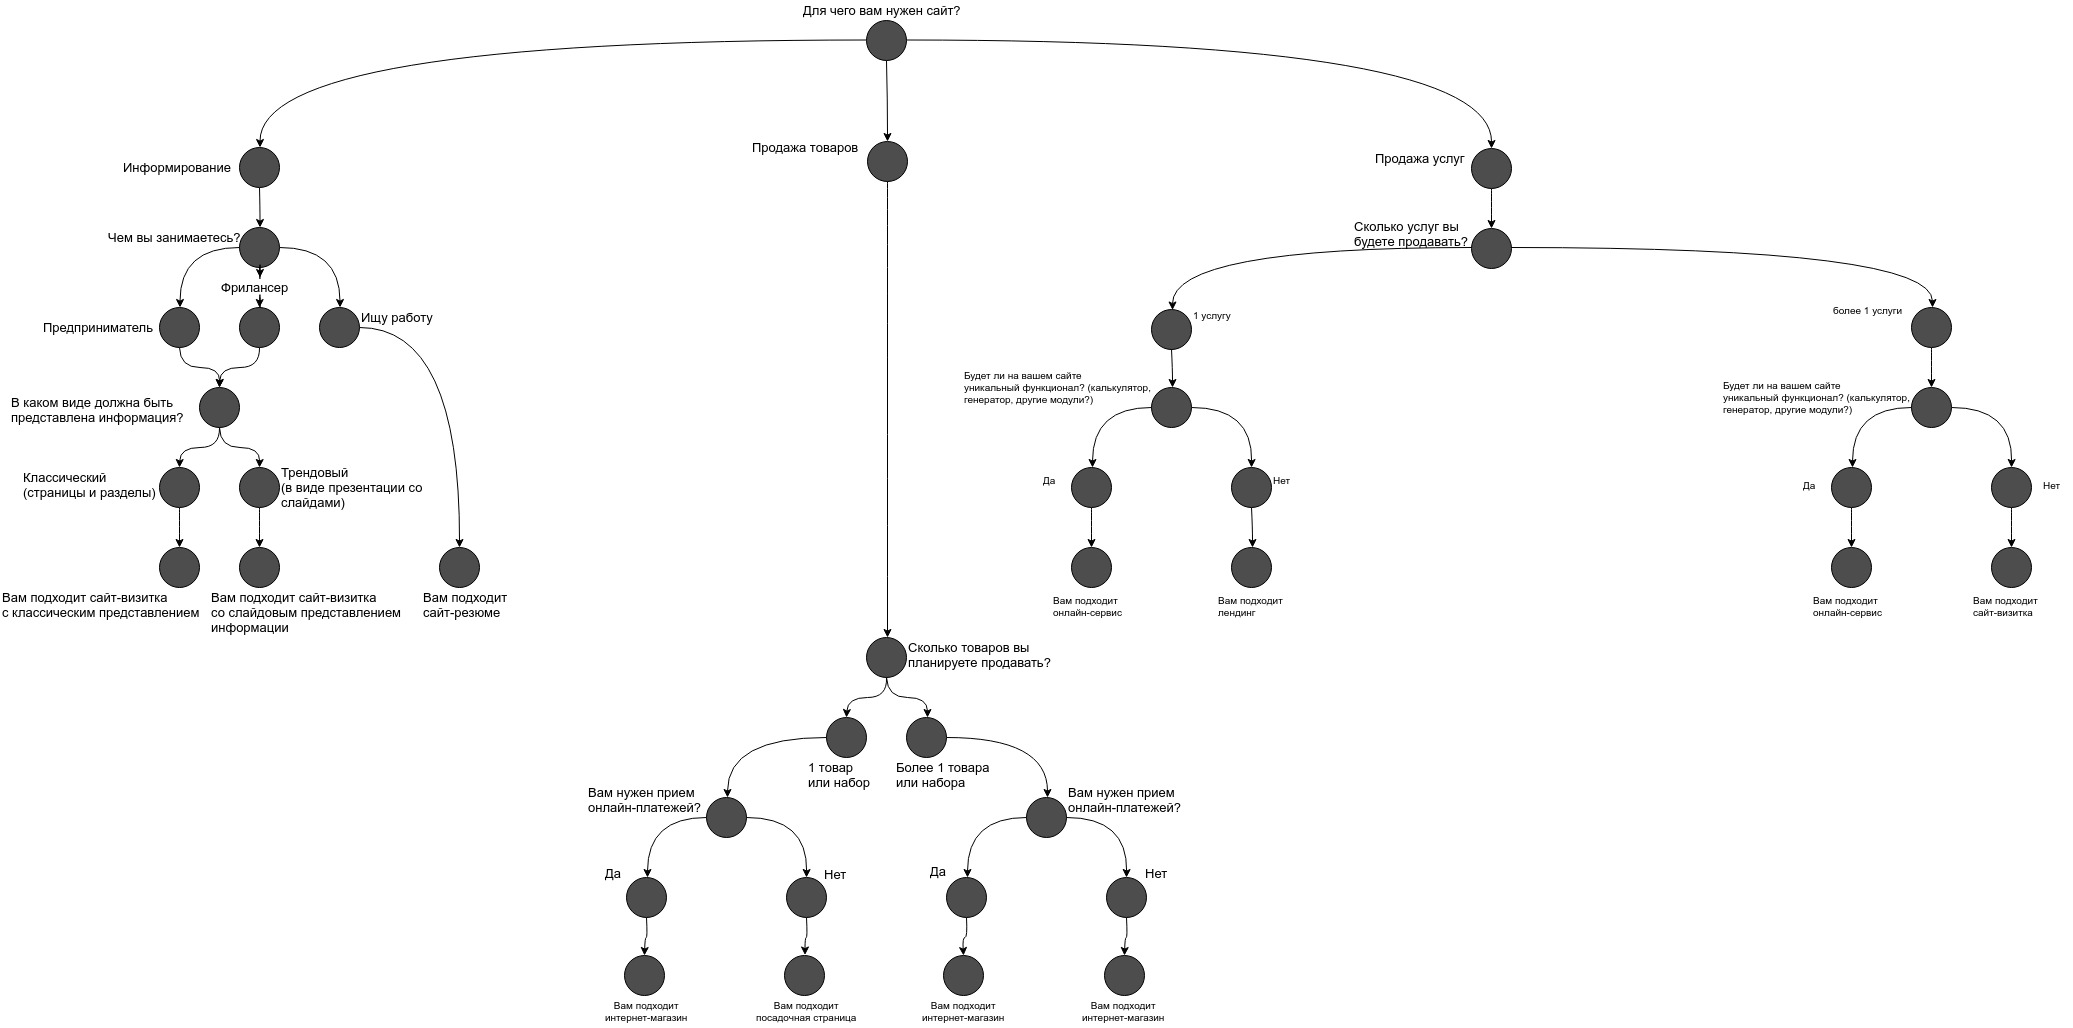
\includegraphics[width=\textwidth]{4-index-0}
  \end{figure}
\end{enumerate}
